% Copyright 2004 by Till Tantau <tantau@users.sourceforge.net>.
%
% In principle, this file can be redistributed and/or modified under
% the terms of the GNU Public License, version 2.
%
% However, this file is supposed to be a template to be modified
% for your own needs. For this reason, if you use this file as a
% template and not specifically distribute it as part of a another
% package/program, I grant the extra permission to freely copy and
% modify this file as you see fit and even to delete this copyright
% notice. 

\documentclass{beamer}

% There are many different themes available for Beamer. A comprehensive
% list with examples is given here:
% http://deic.uab.es/~iblanes/beamer_gallery/index_by_theme.html
% You can uncomment the themes below if you would like to use a different
% one:
%\usetheme{AnnArbor}
\usetheme{Antibes}%talvez
%\usetheme{Bergen}
%\usetheme{Berkeley}%talvez
%\usetheme{Berlin}
%\usetheme{Boadilla}
%\usetheme{boxes}
%\usetheme{CambridgeUS}
%\usetheme{Copenhagen}
%\usetheme{Darmstadt}
%\usetheme{default}
%\usetheme{Frankfurt}%talvez
%\usetheme{Goettingen}
%\usetheme{Hannover}
%\usetheme{Ilmenau}
%\usetheme{JuanLesPins}
%\usetheme{Luebeck}
%\usetheme{Madrid}
%\usetheme{Malmoe}
%\usetheme{Marburg}
%\usetheme{Montpellier}
%\usetheme{PaloAlto}%bomtema
%\usetheme{Pittsburgh}
%\usetheme{Rochester}
%\usetheme{Singapore}
%\usetheme{Szeged}
%\usetheme{Warsaw}

%\usepackage[brazil]{babel}
\usepackage[utf8]{inputenc}
\usepackage[brazil]{babel}
%\usepackage[latin1]{inputenc}
\usepackage{lmodern}
\usepackage{setspace}
\usepackage{verbatim}

% \usepackage{latex8}
\usepackage{subfloat}


\usepackage{algorithm}
\usepackage{algorithmic}
%\usepackage{times}
%\usepackage{amsmath}
%\usepackage{amssymb}
%\usepackage{setspace}
%\usepackage{graphicx}
%\usepackage{indentfirst}
%\usepackage{url}


\title{Criação de clusteres MPI \\no ambiente AWS}

% A subtitle is optional and this may be deleted
%\subtitle{Optional Subtitle}

\author{Celio Henrique Nogueira Larcher Junior}
% - Give the names in the same order as the appear in the paper.
% - Use the \inst{?} command only if the authors have different
%   affiliation.

\institute[Laboratório Nacional de Computação Científica] % (optional, but mostly needed)
{
  Laboratório Nacional de Computação Científica
  %\and
  %\inst{2}%
  %Department of Theoretical Philosophy\\
  %University of Elsewhere
  }
% - Use the \inst command only if there are several affiliations.
% - Keep it simple, no one is interested in your street address.

\date{Petrópolis, 2018}
% - Either use conference name or its abbreviation.
% - Not really informative to the audience, more for people (including
%   yourself) who are reading the slides online

\subject{Ci\^encia da Computa\c{c}~ao}
% This is only inserted into the PDF information catalog. Can be left
% out. 

% If you have a file called "university-logo-filename.xxx", where xxx
% is a graphic format that can be processed by latex or pdflatex,
% resp., then you can add a logo as follows:

%\pgfdeclareimage[height=0.5cm]{university-logo}{figuras/university-logo-ufjf.png}
%\logo{\pgfuseimage{university-logo}}

% Delete this, if you do not want the table of contents to pop up at
% the beginning of each subsection:

% Let's get started
\begin{document}

\begin{frame}
  \titlepage
\end{frame}

\begin{frame}{Agenda}
\footnotesize
  \tableofcontents
  % You might wish to add the option [pausesections]
\end{frame}


\AtBeginSection[]
{
\begin{footnotesize}
  \begin{frame}<beamer>{Agenda}
    \tableofcontents[currentsection,currentsubsection]
  \end{frame}
  \end{footnotesize}
}

% Section and subsections will appear in the presentation overview
% and table of contents.


\section{AWS e aplicação utilizada}

\begin{frame}{Introdução}
	\begin{itemize}
		\item Serviço AWS trás diversas opções para configuração do ambiente computacional
		\item Possibilidade de utilização de um  ambiente computacional distribuído ou maior investimento em uma única instância
		\item Limitações na utilização da conta com categoria estudantil
	\end{itemize}
\end{frame}


\begin{frame}{Aplicação selecionada}
	\begin{itemize}
		\item Utilizado o pacote NAS Parallel Benchmarks
		\item Composto por aplicações desenvolvidas para simulação computacional da dinâmica de fluidos
		\item Diferentes problemas e tamanhos de teste (Classes)
		\item Selecionado o problema LU (Lower-Upper symmetric Gauss-Seidel) na classe C
		\begin{itemize}
			\item Versão modificada do método de Gauss-Seidel para resolução de um sistema de diferenças finitas (Naiver-Stokes 3D)
			\item Tamanho da grid 102 x 102 x 102 e iterações de 250
		\end{itemize}

	\end{itemize}
\end{frame}




\section{Configuração dos clusters MPI}

\begin{frame}{MPI}
	\begin{itemize}
		\item Padrão de comunicação de dados em computação paralela
		\item Diferentes processos executando em paralelo e se comunicando através de mensagens
		\item Implementação nas linguagens de programação mais populares: C/C++, Python, Java, Fortran...
		\item Voltado para paralelização em ambientes distribuídos 
	\end{itemize}
\end{frame}

\begin{frame}[fragile]{Instalação do MPI}
	\begin{itemize}
		\item Utilizado pacote MPICH
		\item Instalação feita em todas as máquinas virtuais participantes do cluster
		\item Processo simples, utilizando-se de apenas alguns comandos:
			\begin{verbatim}		
			sudo apt-get install make gcc g++ gfortran  
			./configure
			make
			sudo make install
			echo "export LD_LIBRARY_PATH=/usr/local/lib" \\
			 >> ~/.bashrc
			sudo reboot
		\end{verbatim}

	\end{itemize}
\end{frame}	
	
\begin{frame}{Chaves RSA}
	\begin{itemize}
		\item Necessário automatizar o acesso das máquinas virtuais entre si
		\item Criação e compartilhamento de uma chave RSA
		\item Acesso inicial às máquinas e adição das mesmas a lista de \textit{hosts} conhecidos
	\end{itemize}	
\end{frame}

\begin{frame}{Configuração das regras de segurança}
	\begin{itemize}
		\item Inserção de todas as instâncias em um mesmo \textit{Security Group}
		\item Liberação das portas para livre conexão entre os membros do \textit{Security Group}
			\begin{figure}[ht]
		\begin{center}
 	 	  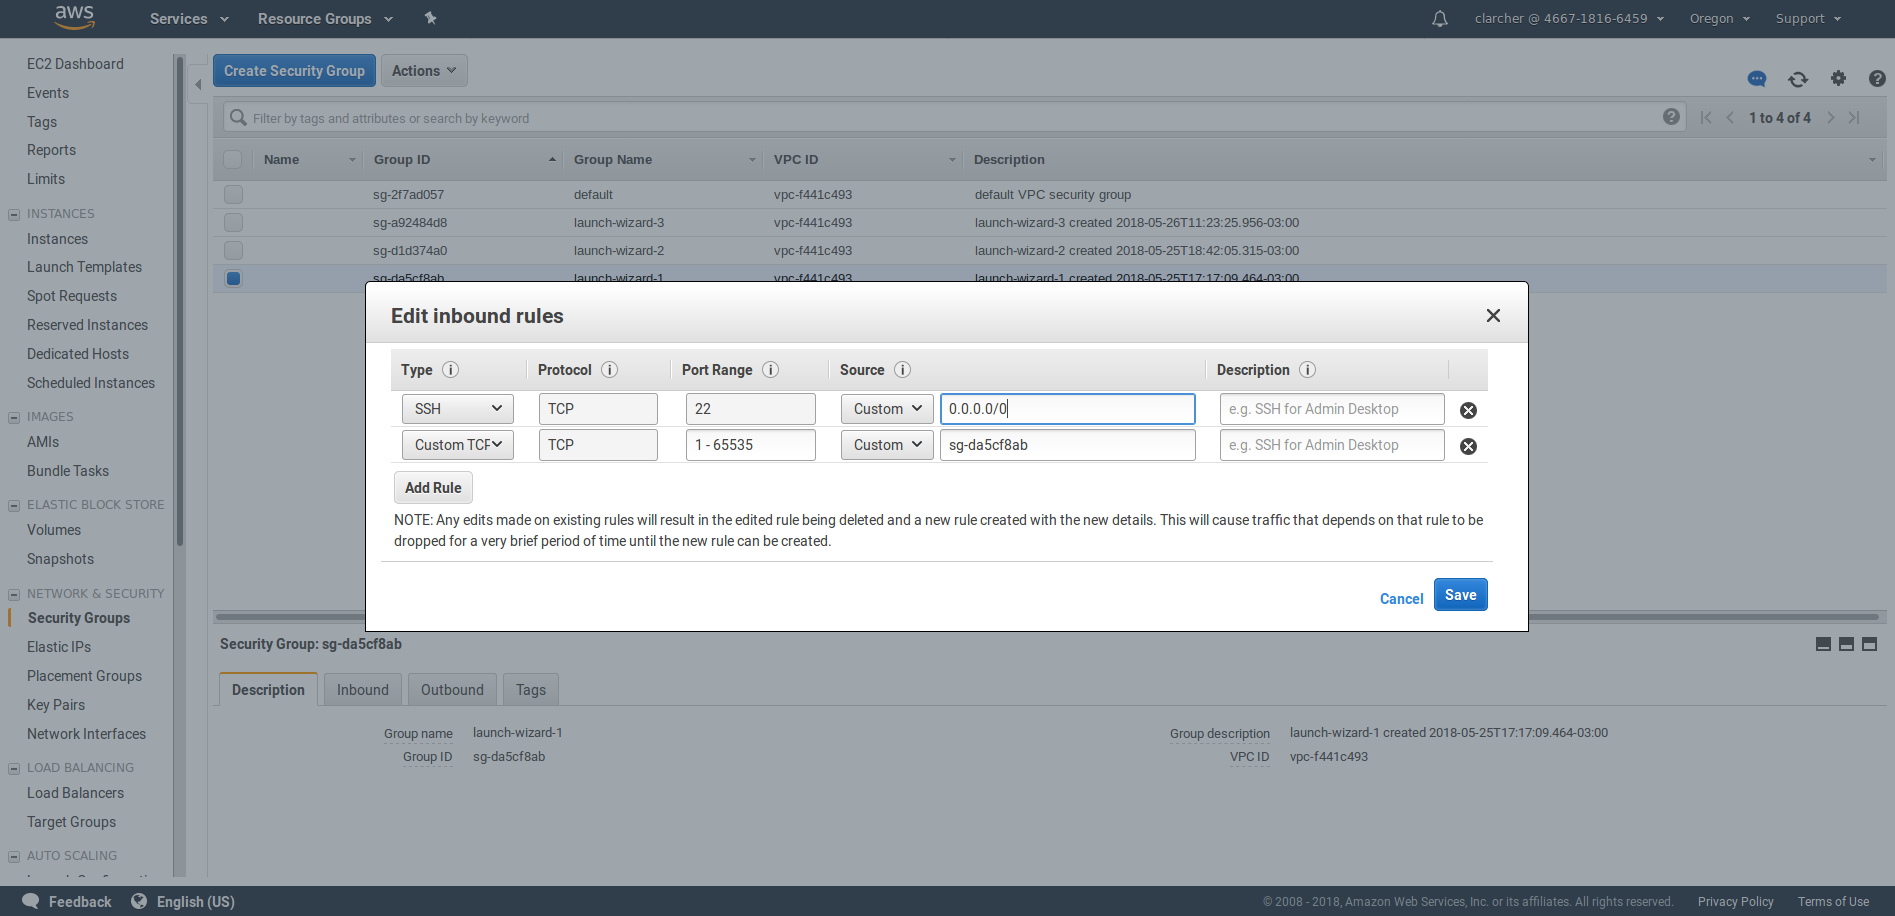
\includegraphics[scale=0.14]{figuras/securitygroup.png}	
		  \label{fig:fluxogramaAG}		
%		  \caption{Tempo de processamento}	  
		\end{center}
	\end{figure}
	\end{itemize}
\end{frame}

\begin{frame}{Configuração de um servidor NFS (Opcional)}
	\begin{itemize}
		\item Instalação e configuração de um servidor NFS em uma das máquinas do cluster
		\item Instalação do cliente NFS nas demais máquinas
		\item Montagem do diretório NFS a ser compartilhado entre as máquinas
	\end{itemize}
\end{frame}

\begin{frame}{Compilação do benchmark}
	\begin{itemize}
		\item Por fim, compilação do \textit{benchmark} em ambiente nuvem
		\item Compartilhamento do executável entre as máquinas do cluster
		\begin{itemize}
			\item Mantendo a mesma estrutura de diretório para acesso ao executável
			\item Copiando  o executável para o diretório NFS
		\end{itemize}
	\end{itemize}
\end{frame}


\section{Experimentação}

\begin{frame}{Configuração dos experimentos}
	\begin{itemize}
		\item Aplicação LU gerada para utilização em 8 processos
		\item Média dos tempos de 5 execuções realizadas em cada cluster
		\item Verificação de desempenho computacional e custo para cada possibilidade 
	\end{itemize}
\end{frame}


\begin{frame}
\begin{table}[htbp]
\center
\small
\caption{Configuração das instâncias utilizadas e preço por instância}
\begin{tabular}{|l|r|r|r|r|}
\hline
 & \multicolumn{1}{c|}{\textbf{vCPU}} & \multicolumn{1}{c|}{\textbf{Mem (GiB)}} & \multicolumn{1}{c|}{\textbf{\$ / hora}} & \multicolumn{1}{l|}{\textbf{Instâncias / cluster}} \\ \hline
t2.micro & 1 & 1 & 0.0116 & 8 \\ \hline
t2.medium & 2 & 4 & 0.0464 & 4 \\ \hline
m4.large & 2 & 8 & 0.1 & 4 \\ \hline
m4.xlarge & 4 & 16 & 0.2 & 2 \\ \hline
t2.2xlarge & 8 & 32 & 0.3712 & 1 \\ \hline
\end{tabular}
\label{tab:inst}
\end{table}
\end{frame}

\begin{frame}
	\begin{figure}[ht]
		\begin{center}
 	 	  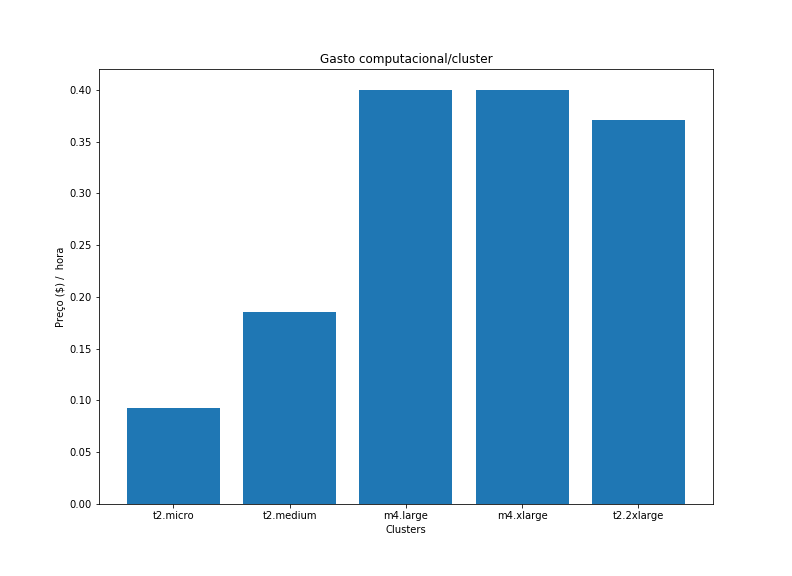
\includegraphics[scale=0.4]{figuras/AllNodesPrecoHora.png}	
		  \label{fig:fluxogramaAG}		
%		  \caption{Tempo de processamento}	  
		\end{center}
	\end{figure}
\end{frame}

\begin{frame}
	\begin{figure}[ht]
		\begin{center}
 	 	  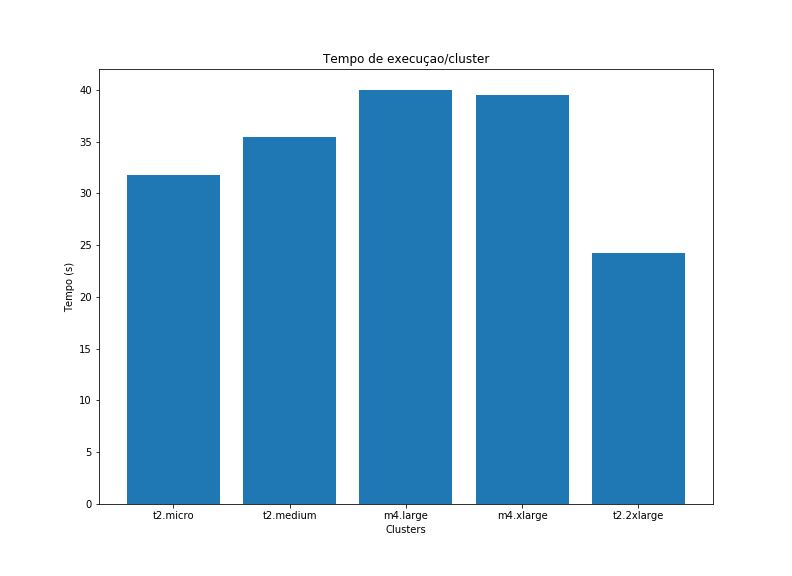
\includegraphics[scale=0.4]{figuras/AllNodesTime.png}	
		  \label{fig:fluxogramaAG}		
%		  \caption{Tempo de processamento}	  
		\end{center}
	\end{figure}
\end{frame}


\begin{frame}
	\begin{figure}[ht]
		\begin{center}
 	 	  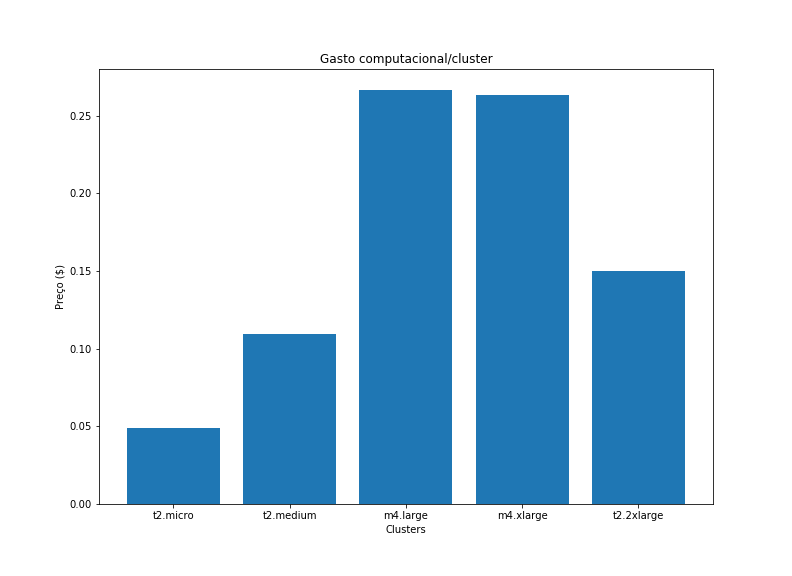
\includegraphics[scale=0.4]{figuras/AllNodesPreco.png}	
		  \label{fig:fluxogramaAG}		
%		  \caption{Tempo de processamento}	  
		\end{center}
	\end{figure}
\end{frame}


\begin{frame}
	\begin{figure}[ht]
		\begin{center}
 	 	  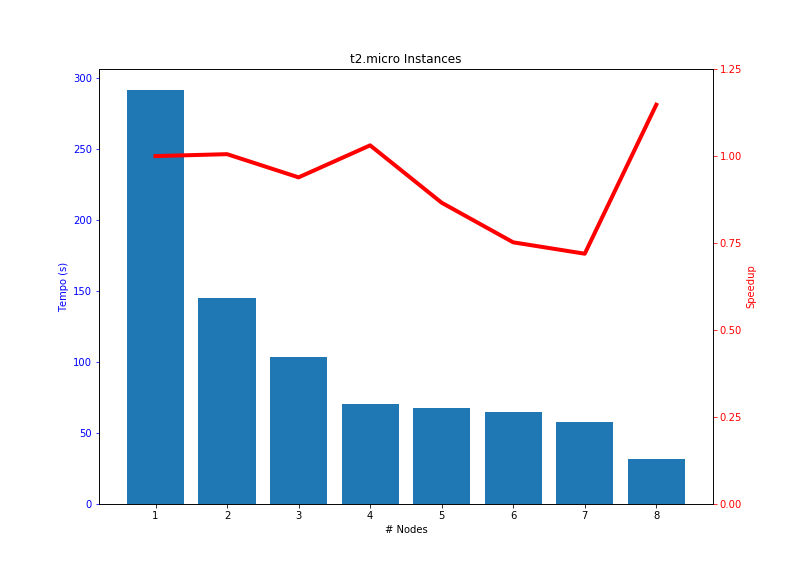
\includegraphics[scale=0.4]{figuras/t2microTime.png}	
		  \label{fig:fluxogramaAG}		
%		  \caption{Tempo de processamento}	  
		\end{center}
	\end{figure}
\end{frame}


\section{Comentários}

\begin{frame}{Comentários}
	\begin{itemize}
		\item Melhor configuração depende muito da aplicação utilizada
		\item Utilização de um cluster MPI, com máquinas de menor capacidade é viável
		\item Em geral, máquina de maior capacidade computacional será melhor escolha
		\item Ainda, as instâncias otimizadas para computação devem ser consideradas
	\end{itemize}
\end{frame}


\section{Refer\^encias}

% All of the following is optional and typically not needed. 
\appendix
\section<presentation>*{\appendixname}
\subsection<presentation>*{Refer\^encias}

\begin{frame}[allowframebreaks]
\scriptsize
  \frametitle<presentation>{Refer\^encias}
    
  \begin{thebibliography}{10}
  
  \beamertemplatearticlebibitems
  % Followed by interesting articles. Keep the list short.     
	
	 \bibitem{AWS}
	Amazon AWS Educate
	\newblock{\em https://www.awseducate.com/student/s/}

	 \bibitem{MPI}
	MPICH 
	\newblock{\em https://www.mpich.org/}


	 \bibitem{NAS}
	NAS Parallel Benchmarks
	\newblock{\em https://www.nas.nasa.gov/publications/npb.html}


	
  \end{thebibliography}
\end{frame}

\begin{frame}
	\begin{center}
	
	\Huge{Obrigado pela atenção!}
	
	\end{center}
\end{frame}

\end{document}
